\section{РАЗРАБОТКА ПРОГРАММНОГО ПРОДУКТА}

Конечный продукт является целостной системой, и необходимо рассказать про каждую ее часть. Ключевым элементом системы является нейронный модуль,
обеспечивающий обработку данных, предоставленных пользователем, с использованием методов нейронного обучения. Поэтому необходимо начать именно с него.
\subsection{Высокоуровневая архитектура нейронного модуля}

Поскольку задача преобразования изображения в текст, выполняемая модулем, не является тривиальной, было решено разбить ее на несколько этапов. 
Схема разбиения представлена на рисунке ~\ref{neuro_model}.

\begin{figure}
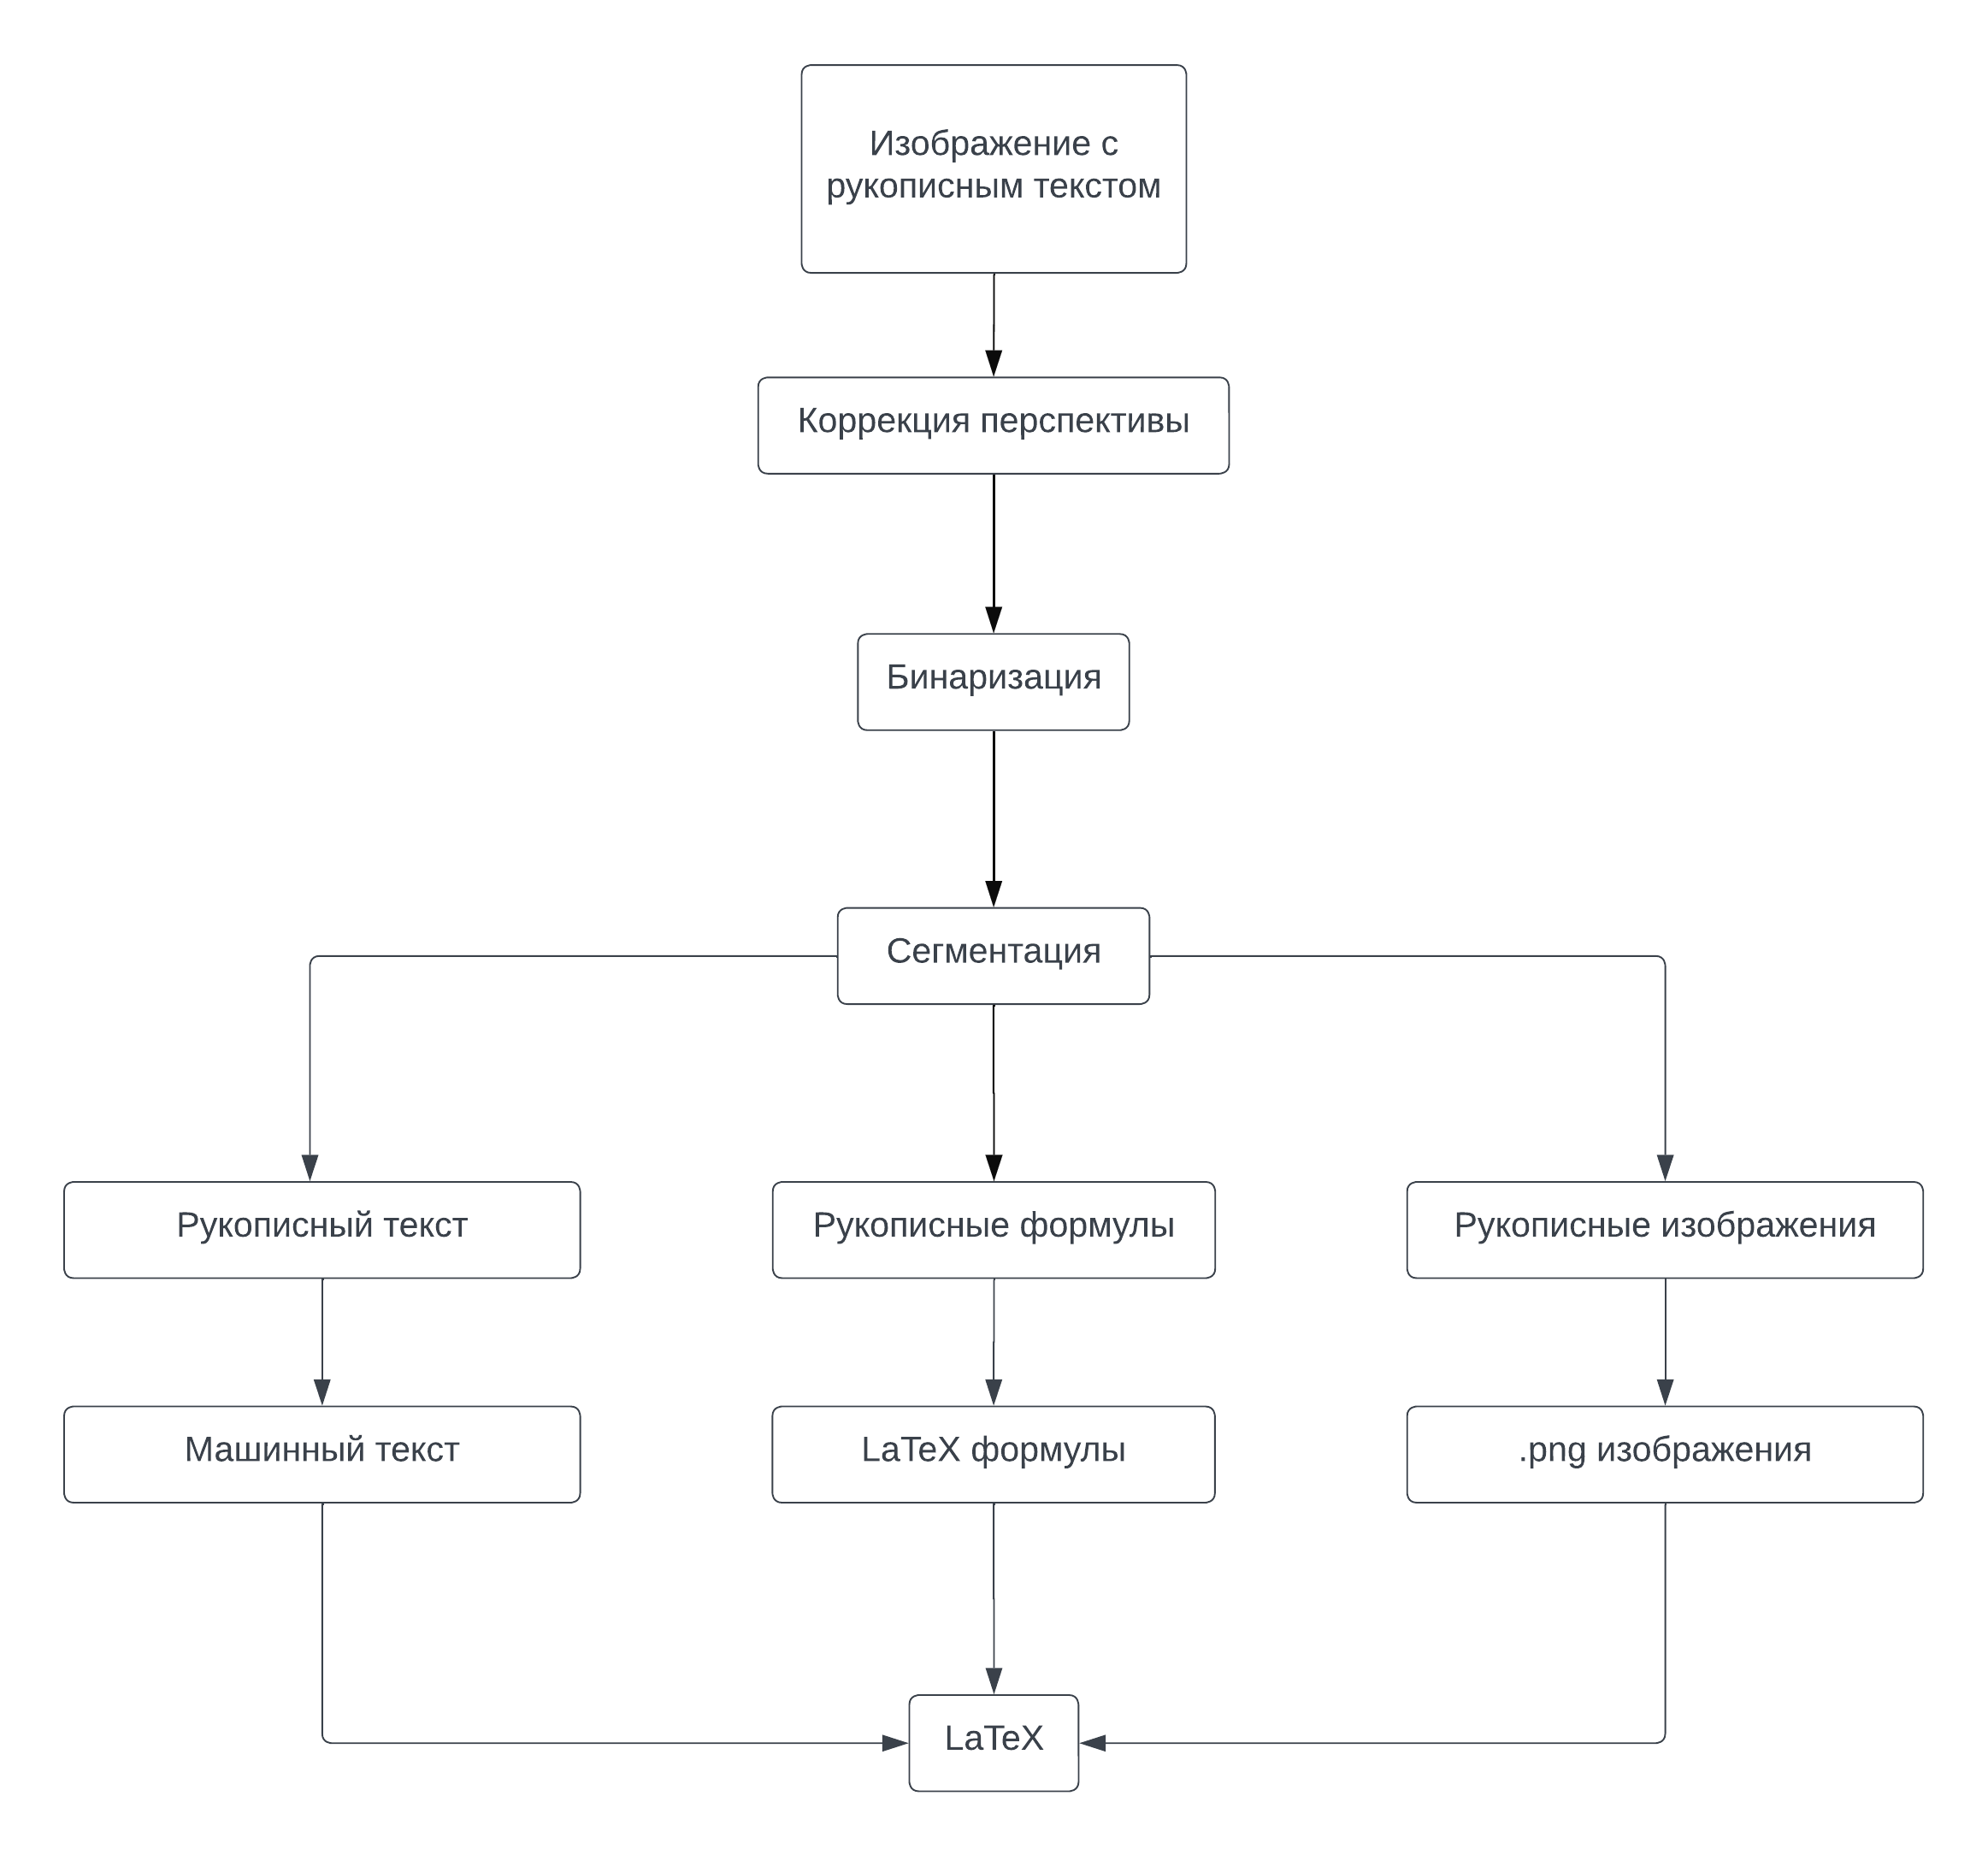
\includegraphics[scale=0.75]{img/Blank_diagram.png}
\caption{Общая архитектура модели}
\label{neuro_model}
\end{figure}

Каждый из этапов данной схемы можно охарактеризовать входными данными и результатом работы модуля (выходными данными).
Такой подход обладает рядом преимуществ:
\begin{itemize}
    \item Гибкость и масштабируемость: модульная структура позволяет легко добавлять новые компоненты или модифицировать существующие без необходимости переписывать всю модель;
    \item Ускорение процесса обучения: благодаря возможности параллельной обработки данных, модульные нейронные сети обучаются быстрее, чем монолитные модели;
    \item Улучшение качества модели: разделение модели на модули позволяет специалистам сосредоточиться на оптимизации каждого компонента, что в итоге приводит к улучшению общей производительности модели;
    \item Простота внедрения новых технологий: модульная архитектура облегчает внедрение новых технологий и подходов, таких как трансфертное обучение или диффузионные модели;
    \item Улучшение производительности: некоторые модули могут исполняться в препроцессинге на клиентской машине, что ослабляет нагрузку на сервер.
\end{itemize}
Однако, имеются и недостатки:
\begin{itemize}
    \item Проблемы с совместимостью: разные модули могут использовать различные архитектуры, форматы данных и методы обучения, что может привести к проблемам совместимости;
    \item Риск ухудшения производительности: неправильно спроектированные или плохо интегрированные модули могут снизить общую производительность модели;
    \item Необходимость в дополнительных ресурсах: для обучения и развертывания модульных моделей часто требуются дополнительные ресурсы, такие как GPU или TPU.
\end{itemize}

Несмотря на недостатки, в современных реалиях важно уметь быстро и без проблем масштабироваться и заменять при необходимости один компонент другим, поэтому было принято решение использовать модульную архитектуру.

Подробнее разберем каждый этап данной схемы.